\definecolor{Purple}{RGB}{120,28,129}
\definecolor{Orange}{RGB}{231,133,50}
\definecolor{Blue}{RGB}{63,96,174}
\definecolor{Red}{RGB}{217,33,32}
\definecolor{Duck}{RGB}{83,158,182}
\definecolor{Green}{RGB}{109,179,136}
\definecolor{Yellow}{RGB}{202,184,67}
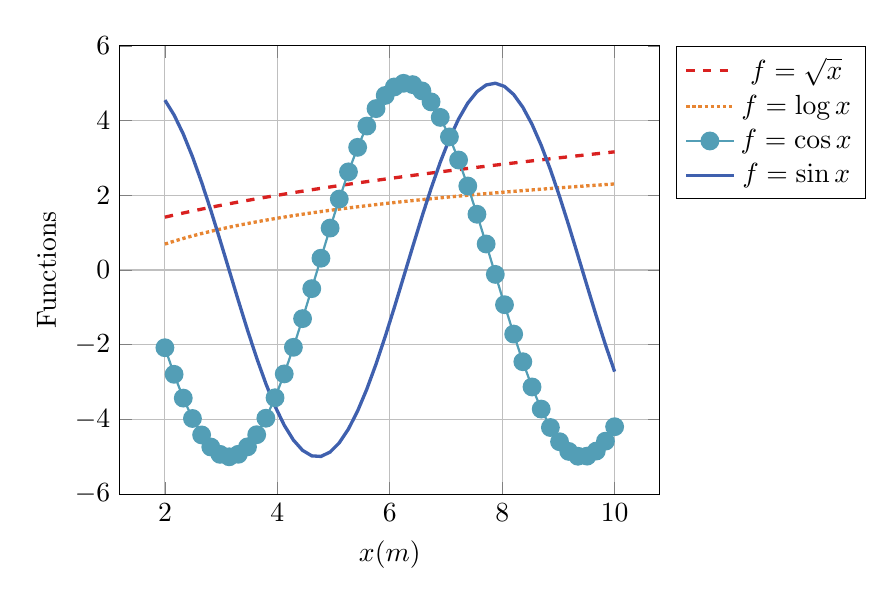
\begin{tikzpicture}[scale=1.]
\begin{axis}[xlabel=$x (m)$,ylabel=Functions,ymajorgrids=true,xmajorgrids=true,legend pos=outer north east,title={}]
\addplot[Red,very thick,mark=none,dashed,mark size=3pt] coordinates {(2.0,1.4142135623730951) (2.163265306122449,1.4708043058552858) (2.326530612244898,1.52529689314733) (2.489795918367347,1.5779087167410373) (2.6530612244897958,1.6288220358559113) (2.816326530612245,1.6781914463529615) (2.979591836734694,1.7261494247992246) (3.142857142857143,1.7728105208558367) (3.3061224489795915,1.8182745801939793) (3.4693877551020407,1.8626292586293283) (3.63265306122449,1.9059520091609048) (3.7959183673469385,1.9483116709979793) (3.9591836734693877,1.9897697538834456) (4.122448979591836,2.030381486221699) (4.285714285714286,2.0701966780270626) (4.448979591836734,2.1092604371762) (4.612244897959183,2.147613768338987) (4.775510204081632,2.1852940772540506) (4.938775510204081,2.2223355980148636) (5.1020408163265305,2.2587697572631282) (5.26530612244898,2.294625486315573) (5.428571428571429,2.32992949004287) (5.591836734693877,2.3647064796066926) (5.755102040816326,2.3989793748209522) (5.918367346938775,2.4327694808466287) (6.081632653061225,2.4660966430902955) (6.244897959183673,2.498979383505129) (6.408163265306122,2.531435020952764) (6.571428571428571,2.5634797778466227) (6.73469387755102,2.5951288749407073) (6.897959183673469,2.626396615835748) (7.061224489795918,2.657296462534039) (7.224489795918367,2.6878411031752543) (7.387755102040816,2.718042512920064) (7.551020408163265,2.747912008810192) (7.7142857142857135,2.7774602993176543) (7.877551020408163,2.806697529198357) (8.040816326530612,2.835633320182744) (8.204081632653061,2.864276807966203) (8.367346938775508,2.892636675902369) (8.53061224489796,2.920721185751553) (8.693877551020407,2.948538205792899) (8.857142857142858,2.9760952365713798) (9.020408163265305,3.0033994345183768) (9.183673469387754,3.0304576336566322) (9.346938775510203,3.0572763655760995) (9.510204081632653,3.083861877846129) (9.673469387755102,3.1102201510110343) (9.83673469387755,3.136356914300021) (10.0,3.1622776601683795) };
\addplot[Orange,very thick,mark=none,densely dotted,mark size=3pt] coordinates {(2.0,0.6931471805599453) (2.163265306122449,0.7716187960014406) (2.326530612244898,0.8443781502838689) (2.489795918367347,0.91220074662263) (2.6530612244897958,0.9757141523449557) (2.816326530612245,1.0354333870465782) (2.979591836734694,1.0917863235977099) (3.142857142857143,1.1451323043030026) (3.3061224489795915,1.1957760371217574) (3.4693877551020407,1.2439781389396352) (3.63265306122449,1.2899632521814586) (3.7959183673469385,1.3339263756025745) (3.9591836734693877,1.3760378609527015) (4.122448979591836,1.4164473992905782) (4.285714285714286,1.455287232606842) (4.448979591836734,1.4926747646784622) (4.612244897959183,1.528714701161659) (4.775510204081632,1.5635008172470748) (4.938775510204081,1.5971174280460598) (5.1020408163265305,1.6296406197516198) (5.26530612244898,1.6611392868109909) (5.428571428571429,1.6916760106710724) (5.591836734693877,1.7213078082774436) (5.755102040816326,1.750086772827487) (5.918367346938775,1.7780606248698931) (6.081632653061225,1.805273188394778) (6.244897959183673,1.831764803841754) (6.408163265306122,1.8575726877976266) (6.571428571428571,1.8827312474337816) (6.73469387755102,1.9072723563498992) (6.897959183673469,1.931225597372392) (7.061224489795918,1.9546184769470976) (7.224489795918367,1.9774766150231478) (7.387755102040816,1.9998239137151443) (7.551020408163265,2.0216827075276433) (7.7142857142857135,2.043073897508961) (7.877551020408163,2.064017071354204) (8.040816326530612,2.084530611187307) (8.204081632653061,2.104631790508394) (8.367346938775508,2.1243368615877265) (8.53061224489796,2.14366113441413) (8.693877551020407,2.1626190481587435) (8.857142857142858,2.181224235989778) (9.020408163265305,2.1994895839670714) (9.183673469387754,2.2174272846537386) (9.346938775510203,2.2350488860035584) (9.510204081632653,2.252365336015019) (9.673469387755102,2.26938702358445) (9.83673469387755,2.2861238159399737) (10.0,2.302585092994046) };
\addplot[Duck,thick,mark=*,solid,mark size=3pt] coordinates {(2.0,-2.080734182735712) (2.163265306122449,-2.792054502196311) (2.326530612244898,-3.429116215309583) (2.489795918367347,-3.9749757721069274) (2.6530612244897958,-4.41511527191081) (2.816326530612245,-4.737828587269876) (2.979591836734694,-4.934532704840567) (3.142857142857143,-4.999996002667765) (3.3061224489795915,-4.932477392509917) (3.4693877551020407,-4.733772626523322) (3.63265306122449,-4.409166536714354) (3.7959183673469385,-3.967292477418361) (3.9591836734693877,-3.4199027091297345) (4.122448979591836,-2.7815558306472927) (4.285714285714286,-2.0692295727155354) (4.448979591836734,-1.3018692514581365) (4.612244897959183,-0.49988389111798315) (4.775510204081632,0.3153965825735388) (4.938775510204081,1.1222886416942863) (5.1020408163265305,1.8993318599753968) (5.26530612244898,2.6258596829438803) (5.428571428571429,3.2825490839311118) (5.591836734693877,3.851934487074578) (5.755102040816326,4.318872288809712) (5.918367346938775,4.670943623251028) (6.081632653061225,4.898784659352287) (6.244897959183673,4.996335645129313) (6.408163265306122,4.961002075264998) (6.571428571428571,4.793723695617932) (6.73469387755102,4.498949509362966) (6.897959183673469,4.084519449510451) (7.061224489795918,3.5614558648894907) (7.224489795918367,2.943670365318029) (7.387755102040816,2.2475938228237) (7.551020408163265,1.4917393695520367) (7.7142857142857135,0.6962100150457378) (7.877551020408163,-0.11783602149584776) (8.040816326530612,-0.9287480437383169) (8.204081632653061,-1.7149587088541398) (8.367346938775508,-2.455557641261106) (8.53061224489796,-3.1308475733953007) (8.693877551020407,-3.7228682221743914) (8.857142857142858,-4.215873967922072) (9.020408163265305,-4.596752631212149) (9.183673469387754,-4.855374209675019) (9.346938775510203,-4.984860299621604) (9.510204081632653,-4.981767036838928) (9.673469387755102,-4.8461766909901085) (9.83673469387755,-4.581695477537261) (10.0,-4.195357645382262) };
\addplot[Blue,very thick,mark=none,solid,mark size=3pt] coordinates {(2.0,4.546487134128409) (2.163265306122449,4.147822519921183) (2.326530612244898,3.638840746982599) (2.489795918367347,3.0330788995940967) (2.6530612244897958,2.346648063886005) (2.816326530612245,1.5978048309002983) (2.979591836734694,0.8064657369404081) (3.142857142857143,-0.00632244465188645) (3.3061224489795915,-0.8189424719591597) (3.4693877551020407,-1.6097815753630935) (3.63265306122449,-2.35780627947216) (3.7959183673469385,-3.0431218179066843) (3.9591836734693877,-3.647501262520289) (4.122448979591836,-4.154870294123759) (4.285714285714286,-4.551734721553914) (4.448979591836734,-4.827539378618038) (4.612244897959183,-4.974948853546209) (4.775510204081632,-4.990042584557864) (4.938775510204081,-4.872419132702357) (5.1020408163265305,-4.625206858691015) (5.26530612244898,-4.254980719755363) (5.428571428571429,-3.771587399435816) (5.591836734693877,-3.1878834212194) (5.755102040816326,-2.5193932112617032) (5.918367346938775,-1.7838962044946904) (6.081632653061225,-1.0009539756126165) (6.244897959183673,-0.19138997155089457) (6.408163265306122,0.623264317297552) (6.571428571428571,1.421342017274927) (6.73469387755102,2.1816171323590967) (6.897959183673469,2.883869079304891) (7.061224489795918,3.5094204824221693) (7.224489795918367,4.041633924584019) (7.387755102040816,4.466354442675228) (7.551020408163265,4.772285998693759) (7.7142857142857135,4.951291913728175) (7.877551020408163,4.998611274347909) (8.040816326530612,4.912985555774844) (8.204081632653061,4.696692094115319) (8.367346938775508,4.355483517411608) (8.53061224489796,3.8984347464289764) (8.693877551020407,3.3377016344071393) (8.857142857142858,2.6881976650903128) (9.020408163265305,1.9671973077056064) (9.183673469387754,1.193876578220163) (9.346938775510203,0.3888030262953284) (9.510204081632653,-0.42661128755002103) (9.673469387755102,-1.230679275727092) (9.83673469387755,-2.002015622095545) (10.0,-2.7201055544468487) };
\legend{$f=\sqrt{x}$,$f=\log{x}$,$f=\cos{x}$,$f=\sin{x}$}
\end{axis}
\end{tikzpicture}